\documentclass[11pt,a4paper]{article}

% Package for displaying figure
\usepackage{graphicx}
\usepackage{caption}
\usepackage{subcaption}

% Package for hyperlinks
\usepackage{hyperref}
\hypersetup{
    colorlinks=true,
    urlcolor=blue
}


% Control the margins
\usepackage[top = 2cm, bottom = 2cm, left = 2cm, right = 2cm]{geometry} 

% Remove paragraph indent
\usepackage{setspace}
\setlength{\parindent}{0in}

% Package to place figures where you want them.
\usepackage{float}

% The fancyhdr package let's us create nice headers.
\usepackage{fancyhdr}

% Import AMS packages
\usepackage{amsmath}
\usepackage{amssymb}
\usepackage{amsfonts}
\DeclareMathOperator*{\argmax}{arg\,max}
\DeclareMathOperator*{\argmin}{arg\,min}

% Import biblatex for reference management
\usepackage{biblatex}
\addbibresource{../references.bib}

% Package for paragraph spacing
\usepackage{parskip}

% Package for code listing
\usepackage{listings}

% Package for inputting pseudocode
\usepackage{algorithm} 
\usepackage{algpseudocode}

% Package for importing csv files as latex tables
\usepackage[l3]{csvsimple}

%%%%%%%%%%%%%%%%%%%%%%%%%%%%%%%%%%%%%%%%%%%%%%%%
% 3. Header (and Footer)
%%%%%%%%%%%%%%%%%%%%%%%%%%%%%%%%%%%%%%%%%%%%%%%%

% To make our document nice we want a header and number the pages in the footer.

\pagestyle{fancy} % With this command we can customize the header style.

\fancyhf{} % This makes sure we do not have other information in our header or footer.

\lhead{\footnotesize Deep Learning: Assessment 3}% \lhead puts text in the top left corner. \footnotesize sets our font to a smaller size.

%\rhead works just like \lhead (you can also use \chead)
\rhead{\footnotesize CCID: 00951537} %<---- Fill in your lastnames.

% Similar commands work for the footer (\lfoot, \cfoot and \rfoot).
% We want to put our page number in the center.
\cfoot{\footnotesize \thepage}

\begin{document}

\thispagestyle{empty} % This command disables the header on the first page. 

\begin{tabular}{p{15.5cm}} % This is a simple tabular environment to align your text nicely 
{\large \bf MLDS: Deep Learning} \\
Imperial College London \\ Spring 2024  \\ CCID: 00951537\\
\hline % \hline produces horizontal lines.
\\
\end{tabular} % Our tabular environment ends here.

\vspace*{0.3cm} % Now we want to add some vertical space in between the line and our title.

\begin{center} % Everything within the center environment is centered.
	{\Large \bf Assignment 3 - Question 4} % <---- Don't forget to put in the right number	
\end{center}  

\vspace{0.4cm}

In the following report, I describe the model and experimental
design choices in training the Vector-Quantized Variational Autoencoder as
described in question 3. I have structured my response below to cover data
processing, model architecture design and experimentation. Finally, I discuss
the potential areas of improvements that I would have liked to explore given
more time.

\section{Data processing}

The exploratory data analysis conducted in question 1 revealed that the Free
Spoken Digit dataset contained the wide variety of recording lengths, amplitude
values and prominent frequencies. My first priority for the project was therefore
to preprocess the data to a format that is more conducive for deep learning.

As a first basic step, I set our to standardize the lengths of the audio entries
by zero padding. Before doing this, I had to remove any files that outliers in terms
of recording length, in order to avoid over dilution of the majority of the dataset
with excessive zero padding. The amplitudes of the resulting data was then scaled
by the standard deviation of the amplitude values.

Next, following the guidance provided in \cite{audio_deep_learning,audio_deep_learning},
I transformed the waveform data into spectrograms using the Short Time Fourier transform
function, implemented in the \verb|tensorflow.signal| library. Spectrogram representations
of sound display the spectral makeup of the signal in terms of frequencies (on the vertical axis)
over time (on the horizontal axis). They can therefore reveal the specific patterns of sound
frequencies that are present in an audio signal that may be more difficult to identify in a 
simple waveform (sound amplitude vs time) representation. The Short Time Fourier Transform
was specifically chosen for this operation due to its robustness to scaling and linear transformations
(meaning that they will be robust to image padding) as well as its revertability (meaning that the model outputs
can be converted back to waveforms and played). The combination of these two properties have made
the SFTF a popular tool in signal analysis and processing \cite{short_time_fourier_transform}.
Figure \ref{fig:spectrogam_digit} shows the magnitude and phase component spectrograms
for one of the audio recordings in the dataset.

\begin{figure}[h]
    \centering
    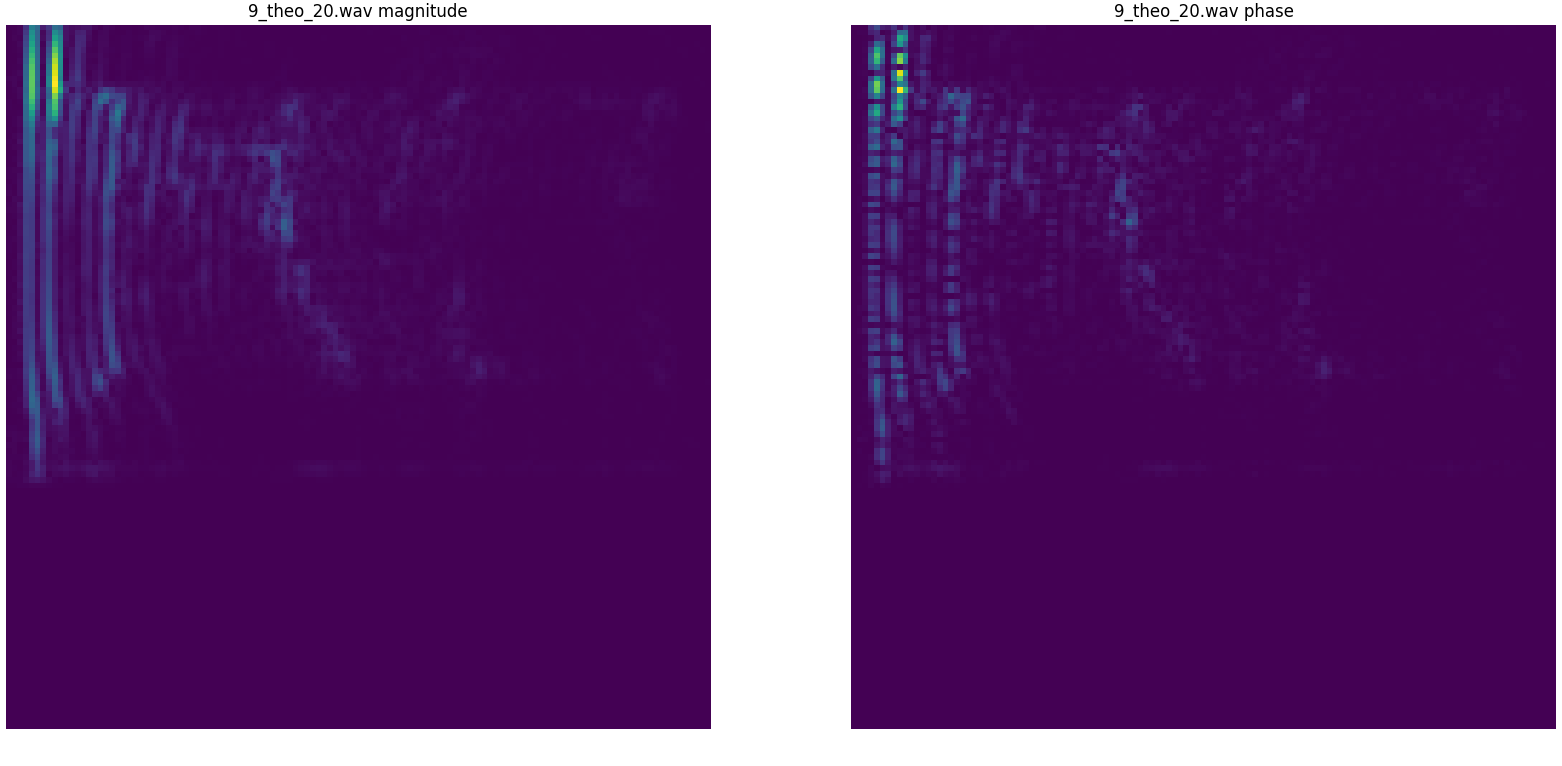
\includegraphics[width=0.8\textwidth]{../figures/spectrograms_digit9_cropped.png}
    \caption{Recording for digit ``nine'', converted to spectrogram by STFT. Left frame shows frequency magnitude, right shows phase.}
    \label{fig:spectrogam_digit}
\end{figure}

\section{Model architecture design}

The transformation of the image into $128 \times 128 \times 2$ tensors meant that the dataset
was transformed to a convenient format in order to be processed by a two-dimensional
Convolutional Neural Network, enabling us to make use of the local connectivity and
equivalence properties of CNNs to help the model identify local features and patterns that are
important for the overall representation of the audio file. 

For question 3a, I therefore start
by adapting the CNN encoder and decoder architecture implemented in \cite{vqvae_keras} to suit
the shape of the spectrogram tensor outputs from the data processing stage. The
encoder for this architecture is first comprised of a two 2D Convolutional layers, the
first with 32 filters and the second with 64. Both layers have a 3-by-3 kernel, ``same''
padding and a stride of 2. Finally, the resulting output is then passed on a
final 2D Convolutional layer with the number of filters equal to our chosen latent dimension
of 128, a kernel size of 1, ``same'' padding and linear activation. The structure of the decoder
is equivalent to the transpose of the encoder architecture. The outputs
of the decoder were then fed into the \verb|RVQVectorQuantizer| layer, which
was implemented changeable hyperparameter inputs for Residual Vector Quantization embedding layers
and $\gamma$. In the next section, I describe the experiments conducted in changing these values.

 

\section{Experimentation}

\begin{figure}[h]
    \centering
    \begin{subfigure}[b]{0.47\textwidth}
        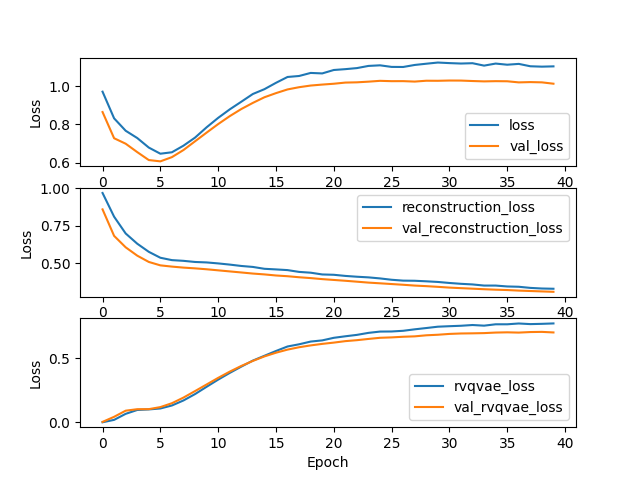
\includegraphics[width = \textwidth]{../figures/model_1_training.png} 
        \subcaption{Model 1 - $\gamma=0.99$, 5 RVQ layers}
        \label{fig:model_1}
    \end{subfigure}
        \hfill
    \begin{subfigure}[b]{0.47\textwidth}
        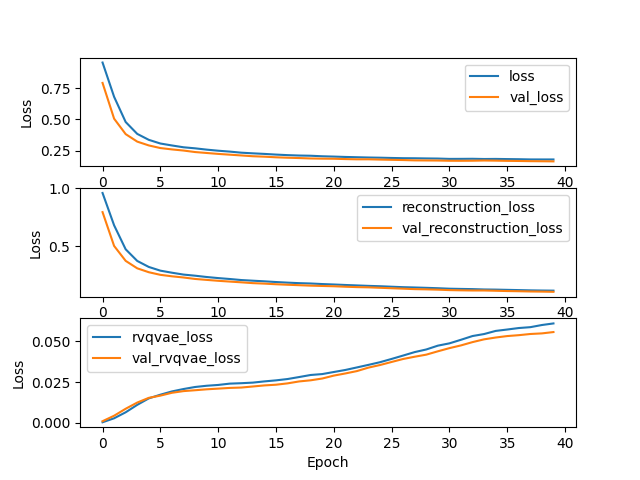
\includegraphics[width = \textwidth]{../figures/model_5_training.png} 
        \subcaption{Model 1 - $\gamma=0.998$, 10 RVQ layers}
        \label{fig:model_5}
    \end{subfigure}
    \caption{Basic and best models from Q3a experimentation}
\end{figure}

In figure \ref{fig:model_1}, I show the training and validation loss for the
basic model architecture as describe in the previous section, with $\gamma = 0.99$
and 5 RVQ layers. The loss curves immediately revealed that the commitment
loss tends to increase rapidly in the early epochs and then plateau later on.
The issue specifically was that increase in commitment loss exceeded the rate
of optimization of the reconstruction loss, leading to an increasing loss for the
majority of the training. For the next few model iterations, I therefore attempted
to find ways in which to improve the optimization of the commitment loss.

My first attempt in doing was to improve the initialization method of
the latent embeddings for the VQVectorQuantizer layer by the use of the
Glorot Normal initialization (Model 2). The reasoning for this was that improved
initialization would lower the rate of commitment loss increase
throughout training. The change did result in an improvement, albeit marginal.

The next attempt was to experiment with the incorporation of a probabilistic
output layer for the decoder model (Model 3), with the reasoning that a stochastic output
may help with regularization throughout training. This however was not the case
as the additional noise created by the probabilistic layer resulted in a deterioration
in loss optimization and quality of reconstructions. Seeing this as a failed attempt,
I ultimately scrapped this approach.

Finally, I sought to improve performance by increasing the latent embedding learning momentum $\gamma$
parameter and number of Residual Vector Quantization layers (in models 4 then 5 respectively).
The combined effect of these two changes were significant. In
figure \ref{fig:model_5}, we see that the training and validation
loss improve continuously throughout all the epochs, a marked improvement
in comparison to figure \ref{fig:model_1}. As a result, the quality of the
audio reconstructions produced by the model were relatively high; not only
was the original audio identifiable in the reconstruction, but the background
interference was also minimal.

\section{Further modifications to explore}

In question 3b, I implemented the RealNVP multiscale framework for producing
a sampling model for the quantized output of the RVQVectorQuantizer layer. 
Unfortunately, my efforts were not particularly successful. As shown
in figure \ref{fig:spectrogam_digit}, the resulting model failed to
produce outputs that captured the local variations in the audio spectrograms.
If I were given more time on this assignment, I would use this to explore the
possible causes for this. Firstly, it is apparent that the data preprocess
bijection suggested in the original paper for image data is not suitable
for RVQVectorQuantizer output, since the range of values for the latter are not
constrained to 0 to 255 pixels. I attempt to account for this in the model by introducing
an extra Sigmoid bijector step or altogether bypassing the preprocess bijector, but this did
not fully solve the issue. The second possible improvement that I would explore
is to increase the size of the model by introducing more affine-squeeze-affine blocks,
to improve the models' ability to capture low and high level features. Lastly,
I would explore the impact of introducing a multi-modal distribution to replace
the unimodal base Gaussian distribution, to reflect the fact that the outputs of
the RVQVectorQuantizer layer are discrete.

\begin{figure}[h]
    \centering
    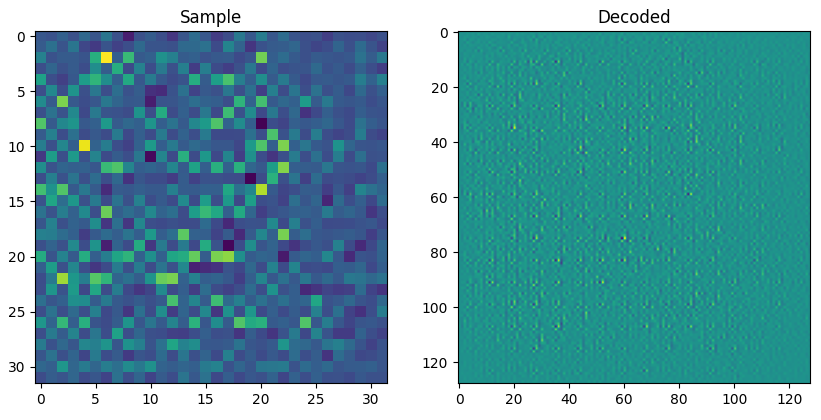
\includegraphics[width=0.5\textwidth]{../figures/spectrogram_sample_0_cropped.png}
    \caption{Sample from the Real NVP model trained on quantized outputs (left) and corresponding output of VQ-VAE decoder (right)}
    \label{fig:spectrogam_digit}
\end{figure}



\printbibliography

\end{document}